\documentclass[11pt,a4paper]{article}
\usepackage[utf8]{inputenc}
\usepackage{amsmath}
\usepackage{amsfonts}
\usepackage{amssymb}
\usepackage{graphicx}
\usepackage[left=2cm,right=2cm,top=2cm,bottom=2cm]{geometry}
\usepackage{authblk}
\usepackage{fancyhdr}
\pagestyle{fancy}
\lhead{Christian Janeczek}
\rhead{\thepage}
\cfoot{Elektronische Marktplätze}
\renewcommand{\headrulewidth}{0.4pt}
\renewcommand{\footrulewidth}{0.4pt}
\title{Elektronische Marktplätze}
\author{Janeczek Christian}
\affil{IT Abteilung am TGM Wien}
\date{\today{}, Vienna}

\begin{document}

\thispagestyle{empty}

\maketitle
\begin{figure}[ht!]
	\centering
	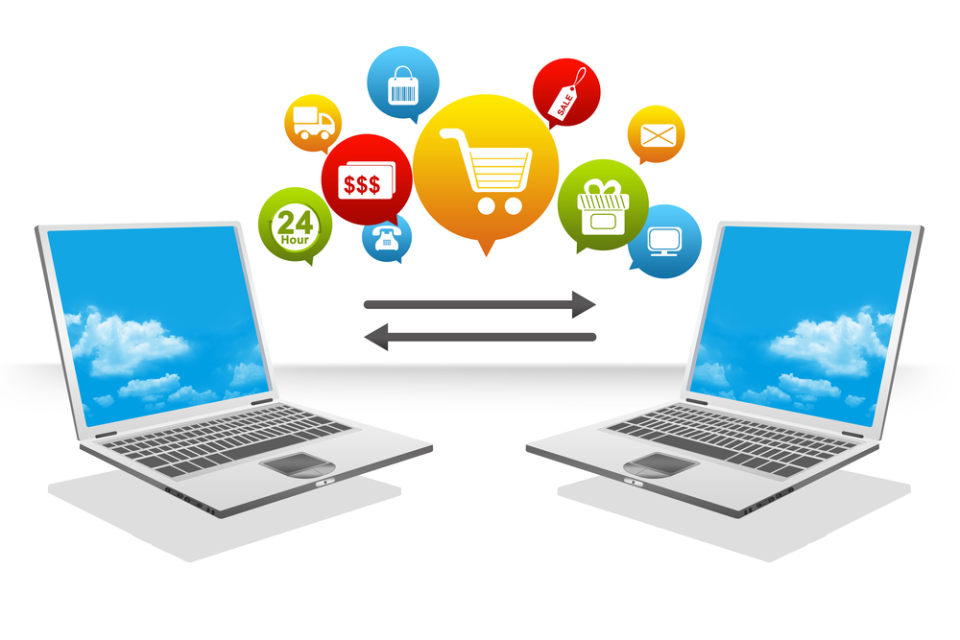
\includegraphics[width=90mm]{elektronischer-handel}
	\caption{Quelle: vistawebcare.com/images/leverage-your-email-marketing.jpg
		\label{elektronischer-handel}}
\end{figure} 
\newpage
\tableofcontents
\newpage

\section{Einleitung}

\textbf{Was ist ein elektronischer Marktplatz?} \newline \newline
Ein elektronischer Marktplatz(EM) oder auch als virtueller Marktplatz bekannt, ist eine elektronische Einkaufsplattform, die es verschiedensten Herstellern, Dienstleistern und Vertriebsunternehmen erleichtert, deren Produkte anzubieten. Diese können von Kunden und Interessenten angesehen sowie erworben werden. \newline
	
\begin{figure}[ht!]
	\centering
	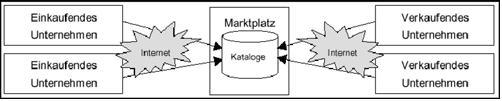
\includegraphics[width=90mm]{eprocurement}
	\caption{Eine konzeptionelle Darstellung eines elektronischen Marktplatzes \label{eprocurement}}
\end{figure}

\noindent Das generelle Konzept eines elektronischen Marktplatzes wird im Abbild 1 erläutert. Eine weitere Aufgabe des EM ist es, die einheitliche Schnittstelle, über welche die einzelnen Transaktionen stattfinden, zu simulieren. Des Weiteren wird eine informationstechnische Unterstützung gewährleistet, die den Handelspartner bei der Auswahl der Dienste und Waren, beim Kauf und bei der Finanzierung unter die Arme greifen soll.

\section{Marktplatz vs. elektronischer Marktplatz}
\textbf{Wieso ist ein elektronischer Marktplatz von Nöten?} \\ \\
In diesem Kapitel werden die einzelnen Unterschiede zwischen einem realen und einem elektronischen Marktplatz erläutert. \\ \\
Eine Elektronik-Fachmarktkette wie MediaMarkt, zum Beispiel, besitzt eine örtliche und zeitliche Gebundenheit. Dies bedeutet, dass sie in einem gewissen Zeitraum an einem bestimmten Ort geöffnet und nur zu seinen Betriebszeiten verfügbar ist. Die Verfügbarkeit eines elektronischen Marktplatzes schlägt die des normalen Marktes um einiges. Elektronische Handelsplätze wie Alibaba, eBay und Amazon bieten eine Nutzbarkeit/Verfügbarkeit von 24/7 (24 Stunden täglich, für 7 Tage die Woche). \\ \\ 
Das Kaufen eines Produkts im örtlichen Elektronik-Markt, ist ohne einem direkten persönlichen Kontakt nahezu unmöglich. Der elektronische Marktplatz hingegen, bietet die Möglichkeit eines Einkaufs mithilfe eines indirekten persönlichen Kontaktes.

\begin{figure}[ht!]
	\centering
	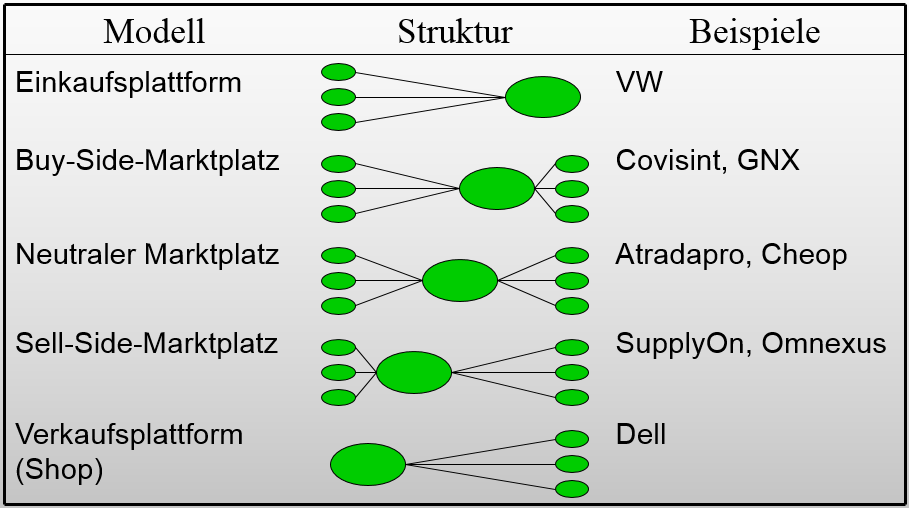
\includegraphics[width=90mm]{classy}
	\caption{Klassifizierung eines elektronischen Marktplatzes \newline Quelle: in Anlehnung an The Boston Consulting Group (2000), S. 13
		 \label{classy}}
\end{figure} 

\newpage

\section{Systemlösungen, Marktplatz Typologien}

\textbf{Welche Arten von elektronischen Marktplätzen gibt es?}
\newline  \newline Man unterscheidet zwischen folgenden E-Market Typologien:

\begin{itemize}
	\item Horizontale Marktplätze
	\item Vertikale Marktplätze
	\item Offene und geschlossene Marktplätze
	\item Zentrale und dezentrale Marktplätze
\end{itemize}

\subsection{Horizontale Marktplätze}

\textbf{Was ist ein Horizontaler Marktplatz?} \newline

\noindent Wenn man von einem horizontalen Marktplatz spricht, wird der branchenübergreifende Marktplatz ins Auge genommen. Die Ausrichtung der HM spezifiziert sich nicht auf einzelne Waren- und Dienstleistungsangebote, sondern wird das Offenstehen für Unternehmen aus den verschiedensten Wirtschaftszweigen gewährleistet. Die Typologie der HM besteht aus einem offenen Nutzerkreis. \newline \newline Als Vergleich kann das klassische amerikanische Kaufhaus genommen werden, da dieses ein großes Repertoire an Services und Waren anbietet. \\

\begin{figure}[ht!]
	\centering
	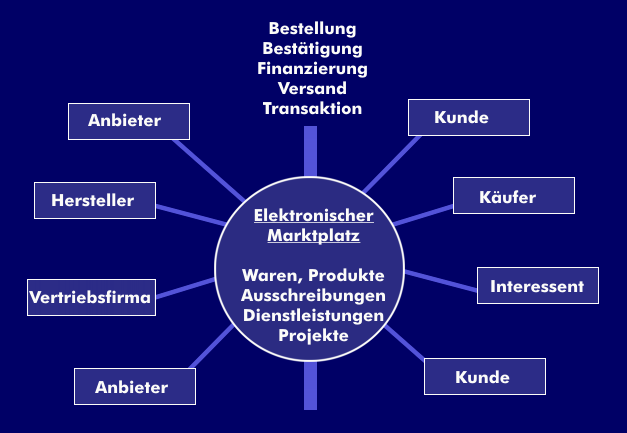
\includegraphics[width=150mm]{hmarktplatz}
	\caption{Die Struktur eines Horizontalen Marktplatzes \label{hmarktplatz}}
\end{figure}

\noindent Sowohl Produkte aus dem Bereich des täglichen Lebens, des Urlaubs, der Mobilität, der Versicherung, der Instandhaltung und der Reparatur werden umfasst. Falls die einzelnen Angebotsbereiche ein zu großes Volumen erreichen sollten, können Vertikale Marktplätze zur Instandhaltung der Übersichtlichkeit verwendet werden.
\newpage
\subsection{Vertikale Marktplätze}
Der wesentliche Unterschied zu der Typologie des Horizontalen Marktplatzes ist jener, dass der Vertikale Marktplatz die Typologie eines branchenspezifischen Angebotssortiments erstrebt. Die Konzentration wird auf bestimmte Branchen und Waren gelegt, dies ist unter Umständen vergleichbar mit Spezialgeschäften. Der Vielfältigkeit von Vertikalen Marktplätzen wird hierbei keine Grenzen gesetzt. Es handelt sich um Güter der Elektronik, Unterhaltungsindustrie, der Holzbearbeitung, des Krankenhausbedarfs, sowie vieles mehr. \\ \\

\noindent Conrad ist ein angesehener vertikaler Marktplatz, welcher sich auf die Branche der Elektronik spezifiert.

\begin{figure}[ht!]
	\centering
	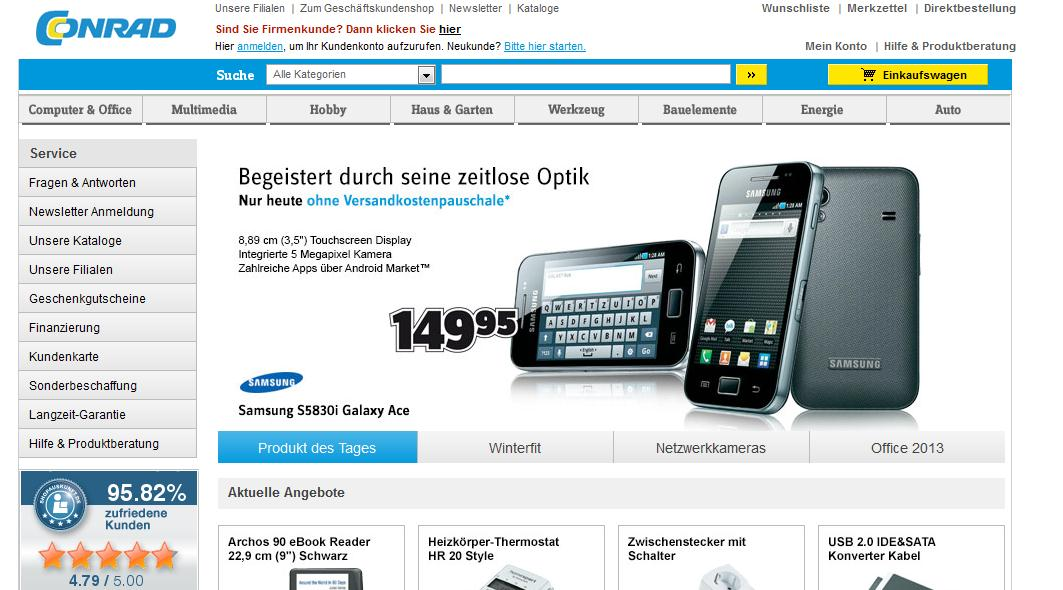
\includegraphics[width=180mm]{conrad}
	\caption{Überblick über das branchenspezifische Angebot Conrads \label{conrad}}
\end{figure}

\noindent Das Ausschlaggebende der vertikalen Struktur ist Electronic Commerce(E-Commerce), eine Methodik der Informatik um den elektronischen Datenaustausch(in unserem Fall geschäftliche Transaktionen) mittels Medien der Elektronik abzuwickeln. Die jeweilige Interaktion und Transaktion kann zwischen Verwaltungen, Unternehmen, Verbrauchern stattfinden, mehr dazu im Kapitel der Teilnehmerbeziehungen. Um Handelspartner mit Statistiken, Produktlebenszyklen, Marktvorhersagen versorgen zu können, findet die E-Collaboration Einsatz.
\begin{figure}[ht!]
	\centering
	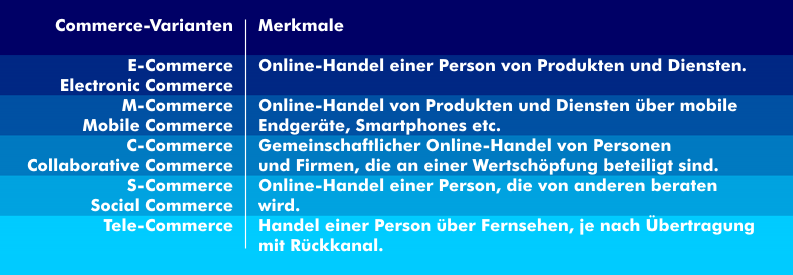
\includegraphics[width=100mm]{e-commerce-varianten}
	\caption{Eine Zusammenfassung der verschiedenen Commerce-Varianten \label{e-commerce-varianten}}
\end{figure}

\newpage

\noindent Des Weiteren werden diese mit für die Kaufentscheidung relevante Informationen gefüttert. Ein mit der Echtzeit arbeitender Marktplatz wäre die Börse, jedoch gibt es neben den genannten elektronischen Handelsplätzen auch noch Marktplätze, die sich auf Ausschreibungen, Auktionen und Versteigerungen konzentrieren. Einer der führenden Marktplätze in diesem Bereich ist eBay und wird dies auch mit großer Wahrscheinlichkeit bleiben.

\begin{figure}[ht!]
	\centering
	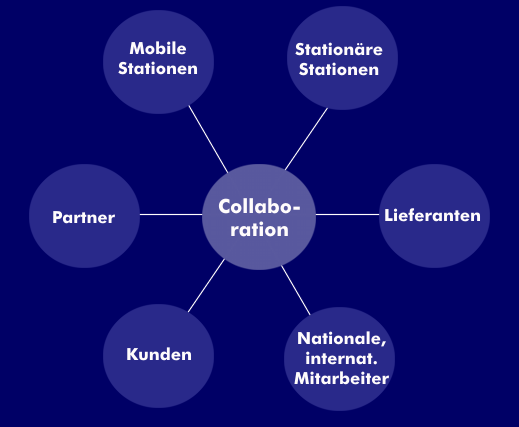
\includegraphics[width=80mm]{collaboration}
	\caption{E-Collaboration bildet die Zusammenarbeit von Gruppen, Teams, verschiedenster Unternehmen und Partner um die Optimierung der Wertschöpfungskette einzuleiten. \label{collaboration}}
\end{figure}
\subsection{Geschlossene und offene Marktplätze}

Spricht man von geschlossenen elektronischen Marktplätzen, bezieht sich dies auf jene, die nur einen bestimmten Kreis von Geschäftspartnern Zugriff verleiht. \newline \newline
Jene elektronischen Marktplätze, die unter dem Namen "offene Marktplätze" bekannt sind, stehen allen Interessenten bereit.
\subsubsection{Zentrale und Dezentrale Marktplätze}

Der Zentrale und Dezentrale Marktplatz unterscheiden sich hinsichtlich ihrer vordefinierten Organisationsstruktur. Erstgenannter basiert auf einem zentralen Rechensystem, welches lokal positioniert ist.

\noindent Beim Dezentralen elektronischen Handelsplatz hingegen herrscht, wie der Name schon sagt, die dezentrale Organisationsstruktur. Die Datenbank des Marktplatzes wird auf viele verschiedene Systeme aufgeteilt. Der Marktbetreiber genießt diese Architektur nicht allzu sehr, wie die Marktteilnehmer, welche die einzelnen Module führen und pflegen. 

\begin{figure}[ht!]
	\centering
	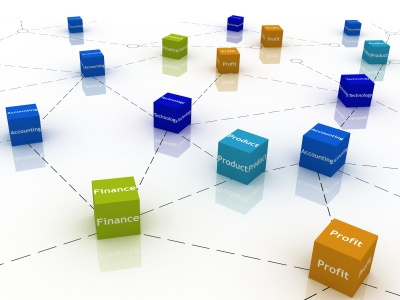
\includegraphics[width=60mm]{filialsteuerung}
	\caption{Folgende Graphik soll eine Dezentrale Organisationsstruktur darstellen \label{filialsteuerung}}
\end{figure}
\newpage
\section{Teilnehmerbeziehungen}
\textbf{Welche Arten von Teilnehmerbeziehungen gibt es?}

\begin{figure}[ht!]
	\centering
	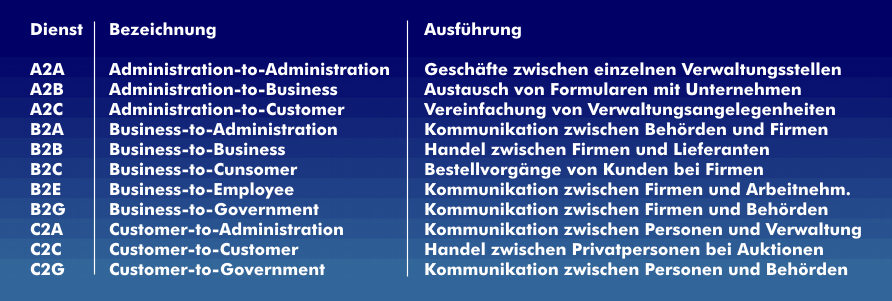
\includegraphics[width=150mm]{teilnehmerbeziehungen}
	\caption{Eine Auflistung aller existierender Teilnehmerbeziehungen bezüglich elektronischen Handels \label{teilnehmerbeziehungen}}
\end{figure}

\noindent Es gibt eine Vielzahl bestehender Teilnehmerbeziehungen im Gebiet des elektronischen Handels, jedoch werden wir uns hier nur an die essentiellen Elemente richten.
\subsubsection{Business-to-Consumer Marktplätze}

Wenn man von einer Teilnehmerbeziehung mit dem Namen "Business-to-Consumer" spricht, wird das E-Commerce zwischen Unternehmen und Endverbraucher unter die Lupe genommen. B2C umfasst den elektronischen Internethandel von Waren oder Dienstleistungen, wie sie im Internet für Endkunden angeboten werden. Die Plattform bietet ein immenses Repertoire an. Diese reicht vom Online-Shopping über den Touristikbereich mit Reisebuchungen, die Reservierung von Tickets und Fahrkarten, über die Dienstleistungen im Finanz- und Versicherungswesen bis hin zu Auktionen. \\ \\

\noindent Falls Ihnen der Begriff Online-Shopping neu sein sollte, hier eine kleine Einführung: Beim Online-Shopping wird analog zu dem Einkauf in Supermärkten mit elektronischen Warenkörben gearbeitet, in die der Kunde seine Ware legen kann. Die ausgewählte Ware wird mit dem kumulierten Preis angezeigt. Es besteht die Möglichkeit die Ware aus dem Warenkorb zu entnehmen. Für das Bezahlen der Ware bestehen wie in einem normalen Geschäft mehrere Möglichkeiten, angefangen von der Kreditkarte, über die Rechnungsstellung, bis hin zum Online-Lastschriftverfahren sowie PayPal.
\subsubsection{Business-to-Business Marktplätze}

B2B ist die Abkürzung für Business-to-Business, welches den elektronischen Internethandel von Waren, Dienstleistungen und Informationen zwischen verschiedenen Unternehmen innerhalb der Wertschöpfungskette umfasst. Um ein kleines Beispiel zu bringen, können B2B-Plattformen im Internet mit Warenbörsen und Großhandelangeboten verglichen werden. \\ \\

\noindent B2B umfasst alle Aktivitäten, die die Wertschöpfungskette tangieren. Man spricht von einer Reihe an Geschäftsprozessen für den Handel mit Waren, Dienstleistungen und Informationen. Dazu gehören auch die Logistik, die Lagerung sowie der Vertrieb und die Transaktionen. Business-to-Business Teilnehmerbeziehungen können zwischen Herstellern, Zulieferern, Vertrieb-, Logistikunternehmen und Kunden stattfinden. Unternehmen erhalten dadurch einen erheblichen Kostenvorteil, da die Kosten für den Einkauf, der Lagerhaltung, des Personals und der Informationen gesenkt werden. Gleichzeitig kann dabei die Produktion und der Vertrieb beschleunigt werden, welches einen auszuwertenden Vorteil bietet.
\subsubsection{Consumer-to-Consumer Marktplätze}

C2C, oder auch Consumer-to-Consumer ist die elektronische Interaktion zwischen Verbrauchern oder Kunden. Man darf es nicht mit dem Begriff Car-to-Car-Communication, welches den Informationsaustausch zwischen fahrenden Fahrzeugen bezeichnet, verwechseln. \\ \\

\noindent Die C2C Teilnehmerbeziehung ist eine weit verbreitete Möglichkeit, die es Verbrauchern erlaubt, ein privates Angebot auf einem elektronischem Marktplatz oder einer ähnlichen Plattform einzutragen. Ein anderer interessierter Verbraucher kann über diese Schnittstelle mit dem Anbieter in Beziehung treten. Es bestehen nun zwei Möglichkeiten: 
\begin{itemize}
	\item Der Marktplatzbetreiber ist an dieser Stelle unmittelbar an der Transaktion beteiligt.
	\item Der Marktplatzbetreiber ist an dieser Stelle nicht an der Transaktion beteiligt.
\end{itemize}

\noindent Dieser gewährleistet lediglich die Infrastruktur für jegliche ein- und ausgehende Transaktionen und erhält Gebühren für das Einstellen des Angebots. \\\\
\noindent Typische C2C-Transaktionen sind Auktionen oder Tauschbörsen. Die berühmtesten Handelsplattformen sind \textit{ciao.de} und die Online-Tauschbörse \textit{e-bay}. Des Weiteren findet der Erfahrungs- und Meinungsaustausch zwischen Kunden und Verbrauchern in Diskussionsforen statt, um dementsprechend Feedback liefern zu können.

\begin{figure}[ht!]
	\centering
	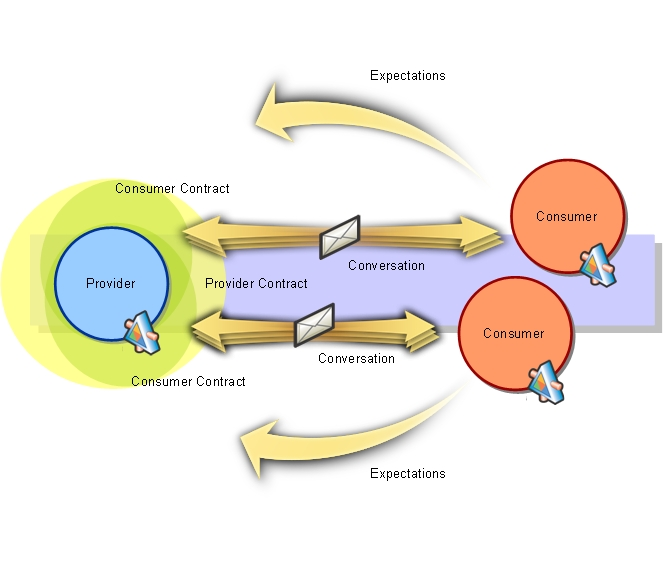
\includegraphics[width=110mm]{consumercc}
	\caption{Quelle: http://martinfowler.com/articles/ConsumerDrivenContracts.jpg \label{consumercc}}
\end{figure}

\begin{figure}[ht!]
	\centering
	
\includegraphics[width=60mm]{ciao}
	\caption{Das derzeitige Logo der Handelsplattform ciao.de \label{ciao}}
\end{figure}

\newpage
\section{Katalogbasierte Systeme und Ausschreibungsplattformen}

\subsection{Katalogbasierte Marktplätze}
\textbf{Was ist ein katalogbasiertes System?} \\ \\
\noindent Katalogbasierte Marktplätze fassen, wie der Name schon sagt, Kataloge verschiedenster Hersteller in einem Gesamtkatalog für ein in der Regel breites Warenspektrum(häufig C-Artikel) zusammen. \\ \\
\textbf{Welche Vorteile hat der Käufer?}
Dem Käufer der Ware wird eine herstellerunabhängige und produktbezogene Suche ermöglicht, welche meistens eine Sammelrechnung und gemeinsame Logistik der bestellten Produkte ist. Ein gutes Beispiel, welches aus dem Büro- und C-Artikel-Bereich genannt werden kann ist: Mercateo

\begin{figure}[ht!]
	\centering
	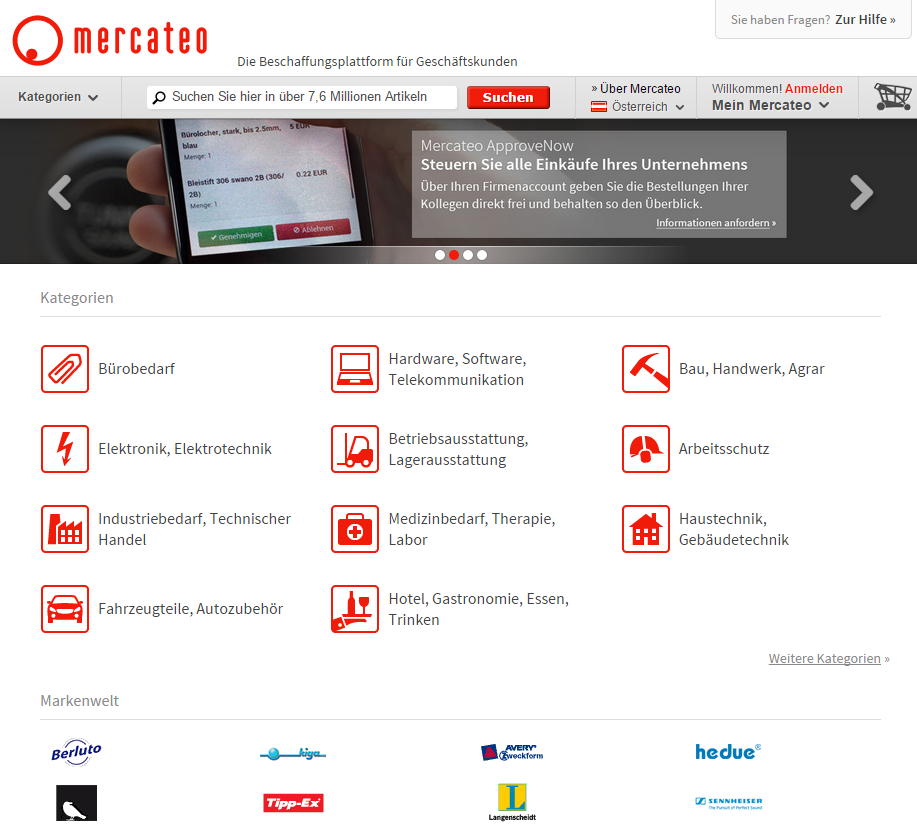
\includegraphics[width=180mm]{mercateo}
	\caption{Die herstellerunabhängige, produktbezogene Katalogübersicht von Mercateo \label{mercateo}}
\end{figure}

\newpage
\todo
\subsection{SAP EBP}

\todo
\subsection{Ausschreibungsplattformen}

\todo
\section{Vergleich vorhandener Märkte}
\newpage
\begin{thebibliography}{1}
	
	\bibitem{definition} DATACOM Buchverlag GmbH {\em Elektronischer Marktplatz}  2012-09-06.
	
	\bibitem{characteristics}  Otto Wettlaufer {\em Electronic Procurement} 2003
	
	\bibitem{norman} E. H. Norman {\em Japan's emergence as a modern
		state} 1940: International Secretariat, Institute of Pacific
	Relations.
	
	\bibitem{fo} Bob Tadashi Wakabayashi {\em Anti-Foreignism and Western
		Learning in Early-Modern Japan} 1986: Harvard University Press.
	
\end{thebibliography}
\section{Quellenangabe}
\subsection{Inhalt}
Einleitung: \\
http://www.itwissen.info/definition/lexikon/Elektronischer-Marktplatz-EM-electronic-marketplace-EM.html \\
Typologien elektronischer Marktplätze: \\
http://www.itwissen.info/definition/lexikon/Elektronischer-Marktplatz-EM-electronic-marketplace-EM.html \\
\subsection{Bilder}
Deckblatt: \\
Einleitung: \\ http://www.vorlesungen.info/sites/default/files/E-Procurement5.JPG \\
Horizontaler Marktplatz: \\
http://www.itwissen.info/bilder/anbieter-kunden-und-funktionen-von-elektronischen-marktplaetzen-em.png
\\ 
http://maxstoreretail.files.wordpress.com/2013/06/filialsteuerung.jpg \\
http://www.itwissen.info/bilder/e-commerce-varianten.png \\
\end{document}
